\chapter{Stakeholders}\label{cha:stakeholders}

\begin{table}[htbp]
\centering
\begin{tabular}{|p{.03\linewidth}|p{.22\linewidth}|p{.12\linewidth}|p{.13\linewidth}|p{.1\linewidth}|p{.1\linewidth}|p{.19\linewidth}|}
\hline
\textbf{Nr} & \textbf{Stakeholder} & \textbf{Company / Institution} & \textbf{Internal / External} & \textbf{Level of Interest} & \textbf{Level of Influence} & \textbf{Potential mgmt strategies} \\ \hline
1  & Employer             & \gls{fhtenl}        & Internal            & Medium            & High               & Keep Satisfied            \\ \hline
2  & Student Workers      & \gls{fhtenl}        & Internal            & Medium            & Low                & Keep Informed             \\ \hline
3  & Pilot Company        & KLG                   & External            & High              & High               & Key Player                \\ \hline
4  & Examiner             & \gls{fhtenl}        & External            & Low               & High               & Keep Satisfied            \\ \hline
5  & Supervising Lecturer & \gls{fhtenl}        & External            & Medium            & Low                & Keep Informed             \\ \hline
6  & Graduation Student   & \gls{fhtenl}        & Internal            & High              & High               & Key Player                \\ \hline
7  & Project Manager      & \gls{fhtenl}        & Internal            & High              & High               & Key Player                \\ \hline
8  & Company Supervisor   & \gls{fhtenl}        & Internal            & High              & High               & Key Player                \\ \hline
9  & Project Team         & \gls{fhtenl}        & Internal            & High              & High               & Key Player                \\ \hline
10 & Partner University   & \gls{hsnr}          & External            & High              & Low                & Keep Informed             \\ \hline
\end{tabular}
\caption{Stakeholder Register}
\label{tab:stakeholder}
\end{table}

\begin{figure}[htbp]
	\centering
	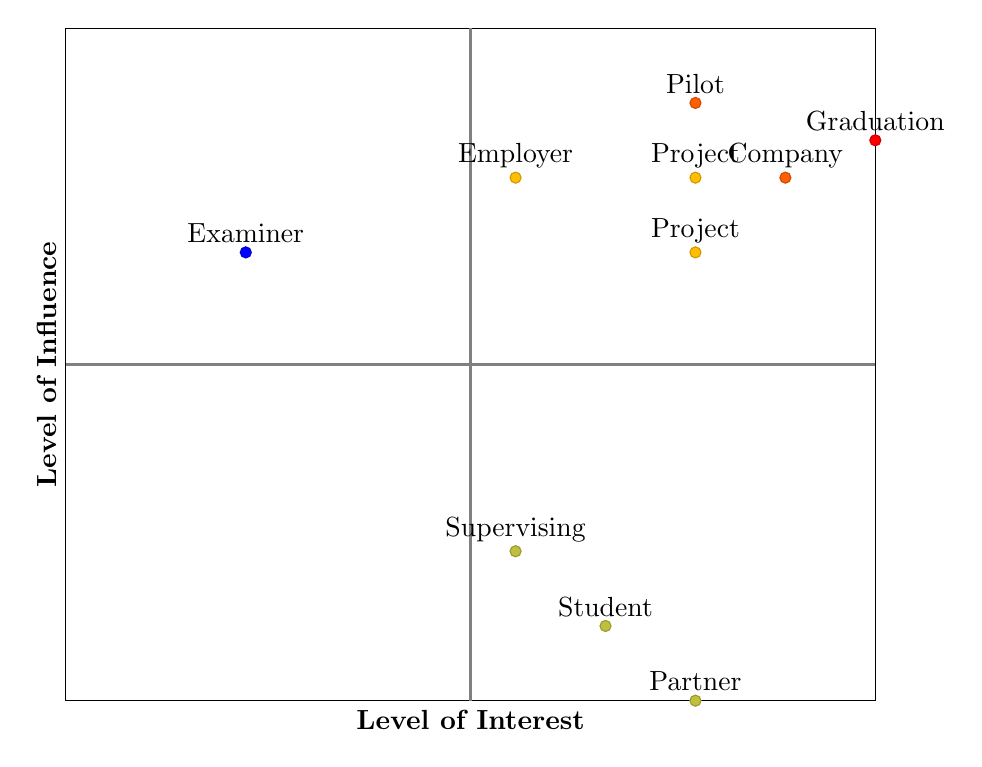
\begin{tikzpicture}
		\begin{axis}[
			scale=1.5,
			xmin=1,
			xmax=10,
			ymin=1,
			ymax=10,
			xtick,
			ytick,
			xlabel=\textbf{Level of Interest},
			ylabel=\textbf{Level of Influence},
			x
			]
			\addplot[
			scatter,
			only marks,
			nodes near coords*={\myvalue},  
			point meta=\thisrow{color},
			visualization depends on={value \thisrow{myvalue} \as \myvalue},
			] table[x=x, y=y]
			{
			x	y	color	myvalue
			6	8	3	Employer
			7	2	2	Student Workers
			8	9	4	Pilot Company 
			3	7	1	Examiner
			6	3	2	Supervising Lecturer
			10	8.5	5	Graduation Student 
			8	8	3	Project Manager 
			9	8	4	Company Supervisor 
			8	7	3	Project Team 
			8	1	2	Partner University
			};
			\addplot[gray,thick, no markers] coordinates {(1,5.5) (10,5.5)};
			\addplot[gray,thick, no markers] coordinates {(5.5,1) (5.5,10)};
		\end{axis}
	\end{tikzpicture}
	\caption{Stakeholder Graph}
	\label{fig:stakeholder}
\end{figure}
\section{Internal Stakeholders}
\section{External Stakeholders}